%!TEX root = modelguide.tex

% Scale latexml image sizes 2x
\newlength{\imglength}
\newcommand{\setlengthLaTeXML}[3]{ %
	\iflatexml %
	\setlength{#1}{#2} %
	\else %
	\setlength{#1}{#3} %
	\fi %
}

\section{Finite Element Models}
\label{FEMModels:sec}

This section details how to construct three-dimensional finite element models,
and how to couple them with the other simulation components described in
previous sections (e.g.~particles and rigid bodies).  Finite element
\emph{muscles}, which have additional properties that allow them to contract
given activation signals, are discussed in Section \ref{sec:fem:muscle}.  An 
example FEM model of the masseter, coupled to a rigid jaw and maxilla, is shown 
in Figure \ref{fig:fem:masseter}.

\begin{figure}[ht]
	\centering
	\setlengthLaTeXML{\imglength}{0.8\textwidth}{0.6\textwidth}
	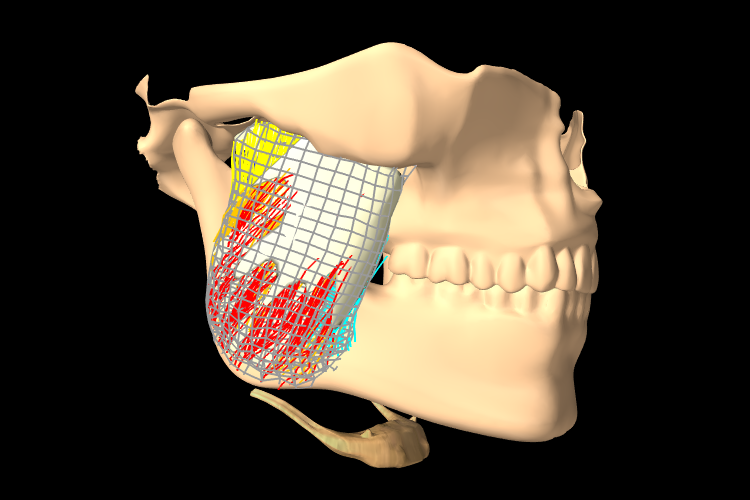
\includegraphics[width=\imglength]{images/fem_masseter}
	\caption{Finite element model of the masseter, coupled to the jaw and 
	         maxilla. \label{fig:fem:masseter}} 
\end{figure}

\subsection{Overview}
\label{sec:fem:overview}

The finite element method (FEM) is a numerical technique used for solving a 
system of partial differential equations (PDEs) over some domain.  The general
approach is to divide the domain into a set of building blocks, referred to
as \emph{elements}.  These partition the space, and form local domains over
which the system of equations can be locally approximated. The corners of these
elements, the \emph{nodes}, become control points in a discretized system.  
The solution is then assumed to be
smoothly interpolated across the elements based on values determined at the
nodes.  Using this discretization, the differential system is converted into 
an algebraic one, which is often linearized and iteratively solved.

In ArtiSynth, the PDEs considered are the governing equations of
continuum mechanics: the conservation of mass, momentum and energy.  To 
complete the system, a \emph{constitutive equation} is required that describes
the stress-strain response of the material.  This constitutive equation is what
distinguishes between material types.  The domain is the three-dimensional space
that the model occupies. This must be divided into small elements which 
accurately represent the geometry. Within each element, the PDEs are
sampled at a set of points, referred to as \emph{integration points}, and 
terms are numerically integrated to form an algebraic system to solve.

The purpose of the rest of this section is to describe the construction and
use of finite elements models within ArtiSynth.  It does not further discuss 
the mathematical framework or theory.
For an in-depth coverage of the nonlinear finite element method, as applied
to continuum mechanics, the reader is referred to the textbook by Bonet and 
Wood \cite{bonet:fem:2000}.

\subsubsection{FemModel3d}
\label{sec:fem:structure}

The basic type of finite element model is implemented in the class 
\javaclass[artisynth.core.femmodels]{FemModel3d}.  This class controls some
properties that are used by the model as a whole.  The key ones that affect
simulation dynamics are:
\begin{center}
	\begin{tabular}{|ll|}
		\hline
		Property & Description\\
		\hline
		{\tt density} & The density of the model\\
		{\tt material} & An object that describes the material's 
		    \emph{constitutive law} (i.e.~its stress-strain relationship).\\
		{\tt particleDamping} & Proportional damping associated with the 
		    particle-like motion of the FEM nodes.\\
		{\tt stiffnessDamping} & Proportional damping associated with the 
		    system's stiffness term.\\
		\hline
	\end{tabular}
\end{center}
These properties can be set and retrieved using the methods
\begin{lstlisting}[]
	setDensity ( double density );    // sets the density
	double getDensity ();             // gets the density

	setMaterial ( FemMaterial mat );  // sets the FEM's material
	FemMaterial getMaterial ();       // gets the FEM's material

	setParticleDamping ( double d );  // sets the particle (mass) damping coefficient
	double getParticleDamping ();     // gets the particle (mass) damping coefficient

	setStiffnessDamping ( double d ); // sets the stiffness damping coefficient
	double getStiffnessDamping ( );   // gets the stiffness damping coefficient
\end{lstlisting}
Keep in mind that ArtiSynth is essentially ``unitless'' (Section 
\ref{sec:mechii:units}), so it is the responsibility of the developer to
ensure that all properties are specified in a compatible way.  

The density of the model is used to compute the mass distribution throughout
the model.  Note that we use a \emph{diagonally lumped mass matrix} (DLMM)
formulation, so the mass is assumed to be concentrated at the location of
the discretized FEM nodes.  To allow for a spatially-varying density,
a mass can later be specified for each node individually.

The FEM's {\tt material} is a delegate object used to compute stress and 
stiffness within individual elements.  It handles the \emph{constitutive}
component of the model.  Materials will be discussed in more detail in
Section \ref{sec:fem:materials}.

The two damping parameters are related to \emph{Rayleigh damping}, which
is used to dissipate energy within finite element models.  There are two 
proportional damping terms: one related to the system's mass, and one related 
to stiffness.  The resulting damping force applied is
\begin{align}
	\f_d & = - (d_M \M + d_K\K)\v,
\end{align}
where $d_M$ is the value of {\tt particleDamping}, $d_K$ is the value of 
{\tt stiffnessDamping}, $\M$ is the FEM model's lumped mass matrix, $\K$ is 
the FEM's stiffness matrix, and $\v$ is the concatenated vector of FEM node
velocities.  Since the lumped mass matrix is diagonal, the mass-related
component of damping can be applied separately to each FEM node.  Thus, the
mass component reduces to the same system as Equation \eqref{eqn:pointdamping},
which is why it is referred to as ``particle damping''.

\subsubsection{Component Structure}

Each \javaclass[artisynth.core.femmodels]{FemModel3d} contains three 
lists of sub-components:

\begin{description}
\item[{\tt nodes}]\mbox{}

The particle-like dynamic components of the model.  These lie at the corners
of the elements and carry all the mass (due to DLMM formulation).

\item[{\tt elements}]\mbox{}

The spatial building blocks of the model.  These define the sub-units over 
which the system is numerically integrated.

\item[{\tt meshes}]\mbox{}

The geometry in the model.  This includes the surface mesh, and any other
embedded geometries.
\end{description}

An example showing each of these components is shown in Figure \ref{fig:fem}.

\begin{figure}[ht]
	\centering
	%\subfigure[][FEM model \label{fig:fem:model}] {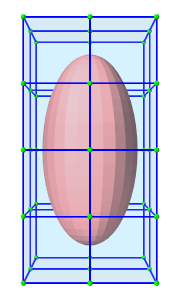
\includegraphics[width=0.2\textwidth]{images/fem_embedded.png}}
	%\subfigure[][Nodes \label{fig:fem:nodes}] {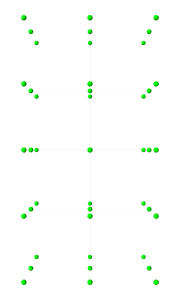
\includegraphics[width=0.2\textwidth]{images/fem_embedded_nodes.png}}
	%\subfigure[][Elements \label{fig:fem:elements}] {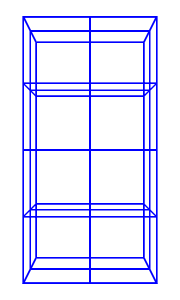
\includegraphics[width=0.2\textwidth]{images/fem_embedded_elements.png}}
	%\subfigure[][Geometry \label{fig:fem:geometry}] {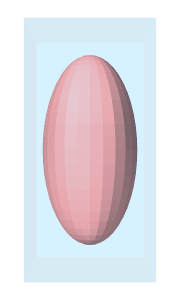
\includegraphics[width=0.2\textwidth]{images/fem_embedded_geometry.png}}
	\setlengthLaTeXML{\imglength}{1.5in}{1.2in}
	\begin{tabular}{cccc}
	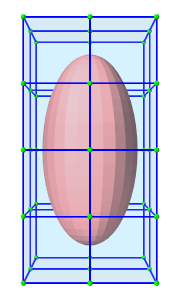
\includegraphics[width=\imglength]{images/fem_embedded.png} & 
	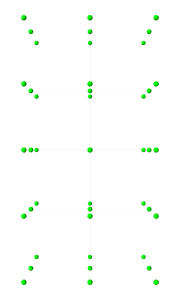
\includegraphics[width=\imglength]{images/fem_embedded_nodes.png} &
	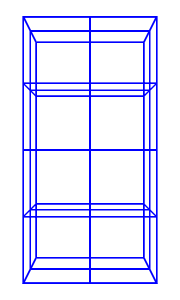
\includegraphics[width=\imglength]{images/fem_embedded_elements.png} &
	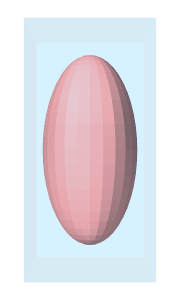
\includegraphics[width=\imglength]{images/fem_embedded_geometry.png}\\
	(a) FEM model & (b) Nodes & (c) Elements & (d) Geometry
	\end{tabular}
	\caption{Sub-components of \javaclass[artisynth.core.femmodels]{FemModel3d}. \label{fig:fem}}
\end{figure}

\paragraph{Nodes}
\ifLaTeXML{\newline}

The set of nodes belong to a finite element model can be obtained by the method
\begin{lstlisting}[]
PointList<FemNode3d> getNodes();  // returns list of FEM nodes
\end{lstlisting}
Nodes are implemented in the class 
\javaclass[artisynth.core.femmodels]{FemNode3d}, which is a subclass of 
\javaclass[artisynth.core.mechmodels]{Particle} (Section 
\ref{ParticlesAndSprings:sec}).  They are the main dynamic components of
the finite element model.  The key properties affecting simulation dynamics
are:
\begin{center}
	\begin{tabular}{|ll|}
		\hline
		Property & Description\\
		\hline
		{\tt restPosition} & The initial position of the node.\\
		{\tt position} & The current position of the node.\\
		{\tt velocity} & The current velocity of the node.\\
		{\tt mass} & The mass of the node.\\
		{\tt dynamic} & Whether the node is considered dynamic or parametric 
		                (e.g.~boundary condition).\\
		\hline
	\end{tabular}
\end{center}
Each of these properties has corresponding {\tt getXxx()} and 
{\tt setXxx(...)} functions to access and modify them.

The {\tt restPosition} property defines the node's position in the FEM model's 
``natural'' or ``undeformed'' state.  Rest positions are used to compute
an initial configuration for the model, from which strains are determined.  A
node's rest position can be updated in code using the method:
\javamethod[artisynth.core.femmodels]{FemNode3d.setRestPosition(Point3d)}.

\begin{sideblock}
If any node's rest positions are changed, the current values 
for stress and stiffness will become invalid.  They can be manually
updated using the method \javamethod[artisynth.core.femmodels] %
{FemModel3d.updateStressAndStiffness()} for the parent model. Otherwise,
stress and stiffness will be automatically updated at the beginning of the 
next time step. 
\end{sideblock}

The properties {\tt position} and {\tt velocity} give the node's current
3D state.  These are common to all point-like particles, as is the 
{\tt mass} property.  Here, however, {\tt mass} represents the lumped mass
of the immediately surrounding material.  Its value is initialized by equally
dividing mass contributions from each adjacent element, given their
densities.  For a finer control of spatially-varying densities,
node masses can be set manually after FEM creation.

The FEM node's {\tt dynamic} property specifies whether or not the 
node is considered when computing the dynamics of the system.  If not,
it is treated as being parametrically controlled.  This has implications
when setting boundary conditions (Section \ref{sec:fem:boundary}).

\paragraph{Elements}
\ifLaTeXML{\newline}

Elements are the spatial building blocks of the domain.  Within each element,
the displacement (or strain) field is interpolated from displacements at nodes:
\begin{align}
	\u(\x) & = \sum_{i=1}^N \phi_i(\x)\u_i, \label{eqn:fem:interp}
\end{align}
where $\u_i$ is the displacement of the $i$th node that is adjacent to the 
element, and $\phi_i(\cdot)$ is referred to as the \emph{shape function} (or 
\emph{basis function}) associated with that node.  Elements are classified by 
their shape, number of nodes, and shape function order (Table 
\ref{tbl:fem:elements}).  ArtiSynth supports the following element types:
\begin{center}
	\setlengthLaTeXML{\imglength}{1.5in}{1in}
	\begin{tabular}{c@{\hspace{5ex}}c@{\hspace{5ex}}c@{\hspace{5ex}}c}
		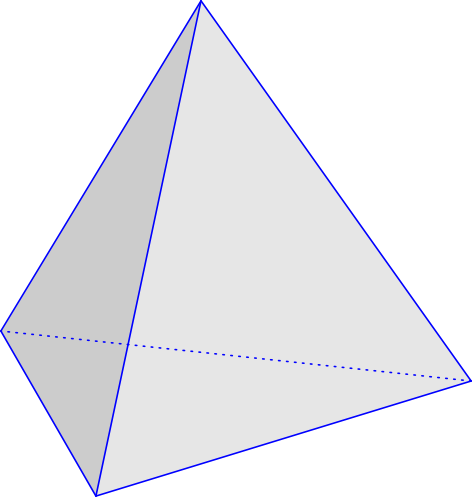
\includegraphics[height=\imglength]{images/fem_element_tet} &
		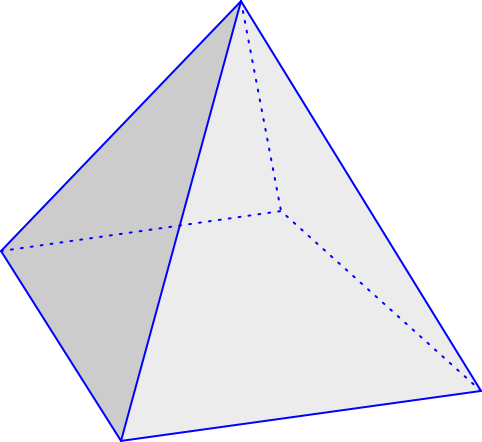
\includegraphics[height=\imglength]{images/fem_element_pyramid} &
		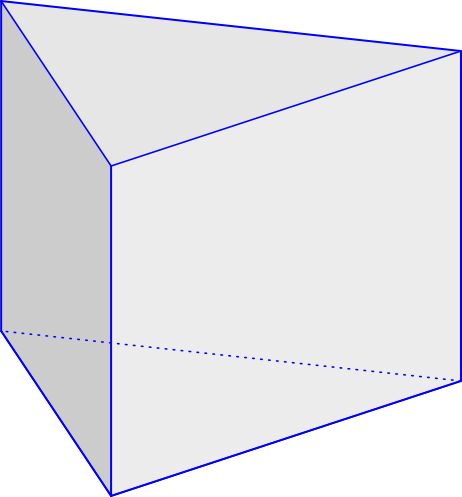
\includegraphics[height=\imglength]{images/fem_element_wedge} &
		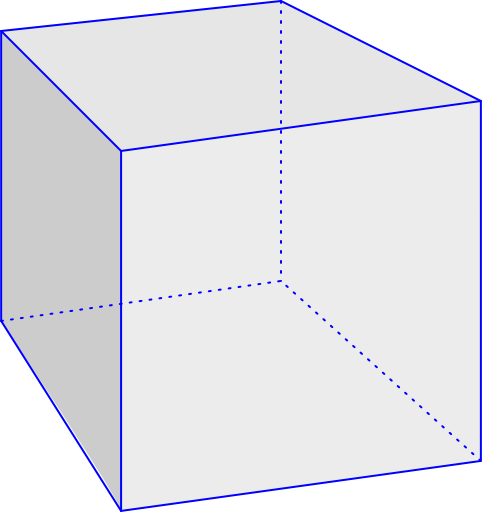
\includegraphics[height=\imglength]{images/fem_element_hex} \\
		\javaclass[artisynth.core.femmodels]{TetElement}, &
		\javaclass[artisynth.core.femmodels]{PyramidElement}, & 
		\javaclass[artisynth.core.femmodels]{WedgeElement}, &
		\javaclass[artisynth.core.femmodels]{HexElement},\\
		\javaclass[artisynth.core.femmodels]{QuadtetElement} &
		\javaclass[artisynth.core.femmodels]{QuadpyramidElement} & 
		\javaclass[artisynth.core.femmodels]{QuadwedgeElement} &
		\javaclass[artisynth.core.femmodels]{QuadhexElement}
	\end{tabular}
\end{center}
The base class for all of these is \javaclass[artisynth.core.femmodels]%
{FemElement3d}.  A numerical integration is performed within each element
to create the (tangent) stiffness matrix.  This integration is performed
by evaluating the stress and stiffness at a set of \emph{integration points}
within each element, and applying numerical quadrature.  The list of elements
in a model can be obtained with the method
\begin{lstlisting}[]
RenderableComponentList<FemElement3d> getElements();  // return the list of elements
\end{lstlisting}

\begin{table}[ht]
\centering
\caption{Supported element types \label{tbl:fem:elements}}
\begin{tabular}{lccc}
	\hline\hline
	Element Type & \# Nodes & Order &  \# Integration Points \\
	\hline
	\javaclass[artisynth.core.femmodels]{TetElement} & 4 & linear & 1\\
	\javaclass[artisynth.core.femmodels]{PyramidElement} & 5 & linear & 5\\
	\javaclass[artisynth.core.femmodels]{WedgeElement} & 6 & linear & 6\\
	\javaclass[artisynth.core.femmodels]{HexElement} & 8 & linear & 8\\
	\javaclass[artisynth.core.femmodels]{QuadtetElement} & 10 & quadratic & 4\\
	\javaclass[artisynth.core.femmodels]{QuadpyramidElement} & 13 & quadratic & 5\\
	\javaclass[artisynth.core.femmodels]{QuadwedgeElement} & 15 & quadratic & 9\\
	\javaclass[artisynth.core.femmodels]{QuadhexElement} & 20 & quadratic & 14\\
	\hline
\end{tabular}
\end{table}

All objects of type \javaclass[artisynth.core.femmodels]{FemModel3d} have the 
following properties:
\begin{center}
	\begin{tabular}{|ll|}
		\hline
		Property & Description\\
		\hline
		{\tt density} & Density of the element\\
		{\tt material} & An object that describes the \emph{constitutive law} 
		                 within the element (i.e.~its stress-strain 
		                 relationship).\\
		\hline
	\end{tabular}
\end{center}

If left unspecified, the element's {\tt density} is inherited from the 
containing {\tt FemModel3d} object.  When set, the mass of the element is
computed and divided amongst all its nodes, updating the lumped mass
matrix.

Each element's' {\tt material} property is also inherited by default from the 
containing {\tt FemModel3d}. Specifying a material here allows for spatially-
varying material properties across the model.  Materials will be discussed
further in Section \ref{sec:fem:materials}.

\paragraph{Meshes}
\ifLaTeXML{\newline}

A geometry inside a finite element model is a mesh that moves along with the
model.  These geometries can be used for visualizations, or for physical 
interactions like collisions.  However, they have no physical properties 
themselves. FEM geometries will be discussed in more detail in Section  
\ref{sec:fem:geometry}.  The list of meshes can be obtained with the method
\begin{lstlisting}[]
MeshComponentList<FemMesh> getMeshes();   // return the list of meshes in a FEM
\end{lstlisting}

\subsubsection{Materials}
\label{sec:fem:materials}

The stress-strain relationship within each element is defined by a ``material''
delegate object, implemented by a subclass of 
\javaclass[artisynth.core.materials]{FemMaterial}.  This material object is 
responsible for implementing the functions:
%
\begin{lstlisting}[]
   public void computeStress (...)  // computes the symmetric stress tensor
   public void computeTangent (...) // computes the local tangent stiffness matrix
\end{lstlisting}
%
Inputs include a deformation gradient, pressure, and a coordinate frame that
specifies any directions of anisotropy. The default material type is 
\javaclass[artisynth.core.materials]{LinearMaterial}, where stress is related 
to strain through:
\begin{gather}
  \sigma(\x) = D\,\epsilon(\x), \label{eqn:fem:mat:linear}\\
  \text{where }\quad D = \begin{bmatrix}
	  \lambda +2\mu & \lambda & \lambda  & 0 & 0 & 0\\
	  \lambda &  \lambda +2\mu & \lambda & 0 & 0 & 0\\
	  \lambda & \lambda & \lambda +2\mu & 0 & 0 & 0\\
	  0 & 0 & 0 & \mu & 0 & 0\\
	  0 & 0 & 0 & 0 & \mu & 0\\
	  0 & 0 & 0 & 0 & 0 & \mu
        \end{bmatrix}, \quad \lambda = \dfrac{E\nu}{(1+\nu)(1-2\nu)},  \quad
      \mu = \dfrac{E}{2(1+\nu)},\notag
\end{gather}
$\sigma$ is the standard $6\times 1$ stress vector, $\epsilon$ is the 
strain vector, $E$ is the Young's Modulus, and $\nu$ is Poisson's ratio. This
linear material uses a corotational formulation, so rotations are removed
per element before computing the strain \cite{ngan:fem:2008}.  To enable or
disable this corotational formulation, use 
\javamethod[artisynth.core.materials]{LinearMaterial.setCorotated(boolean)}.

Other, non-linear, models are available in the package  
{\tt artisynth.core.materials}.  A list of common materials is provided in 
Table \ref{tbl:fem:materials}.  Those that are subclasses of 
\javaclass[artisynth.core.materials]{IncompressibleMaterial} allow for 
incompressibility.

\begin{table}[ht]
	\centering
 	\caption{Commonly used FEM materials \label{tbl:fem:materials}}
 	\begin{tabular}{|lll|}
 		\hline
 		\hline
 		Material & Parameters & \\
 		\hline
 		\javaclass[artisynth.core.materials]{LinearMaterial} & $E$ & Young's modulus \\
 		& $\nu$ & Poisson's ratio\\
 		& corotated & corotational formulation\\
 		\hline
 		\javaclass[artisynth.core.materials]{StVenantKirchoffMaterial} & $E$ & Young's modulus\\
 		& $\nu$ & Poisson's ratio\\
 		\hline
 		\javaclass[artisynth.core.materials]{NeoHookeanMaterial} & $E$ & Young's modulus\\
 		& $\nu$ & Poisson's ratio\\
 		\hline
 		\javaclass[artisynth.core.materials]{IncompressibleNeoHookeanMaterial} & $G$ & shear modulus\\
 		& $\kappa$ & bulk modulus\\
 		\hline
 		\javaclass[artisynth.core.materials]{MooneyRivlinMaterial} & $C_{10},C_{01},C_{20},C_{02}$ & distortional parameters\\
 		& $\kappa$ & bulk modulus\\
 		\hline
 		\javaclass[artisynth.core.materials]{OgdenMaterial} & $\mu_1,\ldots,\mu_6$ & material parameters\\
 		& $\alpha_1,\ldots,\alpha_6$ &\\
 		& $\kappa$ & bulk modulus\\
		\hline
	\end{tabular}
\end{table}


\subsubsection{Boundary conditions}
\label{sec:fem:boundary}

Boundary conditions can be implemented in one of several ways:
\begin{enumerate}
	\item Explicitly setting FEM node positions/velocities
	\item Attaching FEM nodes to other dynamic components
	\item Enabling collisions
\end{enumerate}
To enforce an explicit (Dirichlet) boundary condition for a set of  
nodes, their {\tt dynamic} property must be set to {\tt false}.  This notifies
ArtiSynth that the state of these nodes (both position and velocity) will 
be controlled parametrically.  By disabling dynamics, a fixed 
boundary condition is applied.  For a moving boundary, positions and velocities 
of the boundary nodes need to be explicitly set every timestep.  This can be 
accomplished with either a \javaclass[artisynth.core.modelbase]{Controller} 
(Section \ref{ControllersAndMonitors:sec}) or an 
\javaclass[artisynth.core.probes]{InputProbe} (Section \ref{Probes:sec}).
Note that both the position \emph{and} velocity of the nodes should be
explicitly set for consistency.

Another type of supported boundary condition is to attach FEM nodes to other
components, including particles, springs, rigid bodies, and locations within
other FEM elements.  Here, the node is still considered dynamic, but its
motion is coupled to that of the attached component through a constraint
mechanism. Attachments will be discussed further in Section 
\ref{sec:fem:nodeattachments}.

Finally, the boundary of a FEM can be constrained by enabling collisions
with other components.  This will be covered in Section
\ref{sec:fem:collision}.


\subsection{FEM model creation}

Creating a finite element model in ArtiSynth typically follows the pattern:
\begin{lstlisting}[]
   // Create and add main MechModel
   MechModel mech = new MechModel("mech");
   addModel(mech);
      
   // Create FEM
   FemModel3d fem = new FemModel3d("fem");
   
   /* ... Setup FEM structure and properties ... */
   
   // Add FEM to model
   mech.addModel(fem); 
\end{lstlisting}
The main code block for the FEM setup should do the following:
\begin{itemize}
	\setlength{\itemsep}{-0.3em}
	\item Build the node/element structure
	\item Set physical properties%
	\ifLaTeXMLelse{}{\vspace{-0.5em}}
	\begin{itemize}
		\setlength{\itemsep}{-0.3em}
		\item density
		\item damping
		\item material
	\end{itemize} 
	\item Set boundary conditions
	\item Set render properties
\end{itemize}
Building the FEM structure can be done with the use of factory
methods for simple shapes, by loading external files, or by writing code
to manually assemble the nodes and elements.

\subsubsection{Factory methods}

For simple shapes such as beams and ellipsoids, there are factory methods to 
automatically build the node and element structure.  These methods are found
in the \javaclass[artisynth.core.femmodels]{FemFactory} class.  Some common
methods are
\begin{lstlisting}[]
FemFactory.createGrid(...)          // basic beam
FemFactory.createCylinder(...)      // cylinder
FemFactory.createTube(...)          // hollowed cylinder
FemFactory.createEllipsoid(...)     // ellipsoid
FemFactory.createTorus(...)         // torus
\end{lstlisting}
The inputs specify the dimensions, resolution, and potentially the type
of element to use.  The following code creates a basic beam made up of
hexahedral elements:
\begin{lstlisting}[]
// Create FEM
FemModel3d beam = new FemModel3d("beam");
      
// Build FEM structure
double[] size = {1.0, 0.25, 0.25};  // widths
int[] res = {8, 2, 2};              // resolution (# elements)
      
FemFactory.createGrid(beam, FemElementType.Hex,
	size[0], size[1], size[2], 
	res[0], res[1], res[2]);

/* ... Set FEM properties ... */

// Add FEM to model
mech.addModel(beam);
\end{lstlisting}

\subsubsection{Loading external FEM meshes}

For more complex geometries, volumetric meshes can be loaded from external
files.  A list of supported file types is provided in Table 
\ref{tbl:fem:fileformats}. To load a geometry, an appropriate file reader
must be created.  Readers capable of reading FEM models implement the 
interface \javaclass[artisynth.core.femmodels]{FemReader}, which has the
method
\begin{lstlisting}[]
readFem( FemModel3d fem )   // populates the FEM based on file contents
\end{lstlisting}
Additionally, many {\tt FemReader} classes have static methods to handle
the loading of files for convenience.

\begin{table}[ht]
	\centering
	\caption{Supported FEM geometry files \label{tbl:fem:fileformats}}
	\begin{tabular}{llll}
		\hline\hline
		Format & File extensions & Reader & Writer\\
		\hline
		ANSYS & .node, .elem & \javaclass[artisynth.core.femmodels]{AnsysReader} & \javaclass[artisynth.core.femmodels]{AnsysWriter}\\
		TetGen & .node, .ele & \javaclass[artisynth.core.femmodels]{TetGenReader} & \javaclass[artisynth.core.femmodels]{TetGenWriter}\\
		Abaqus & .inp & \javaclass[artisynth.core.femmodels]{AbaqusReader} & \javaclass[artisynth.core.femmodels]{AbaqusWriter}\\
		VTK (ASCII) & .vtk & \javaclass[artisynth.core.femmodels]{VtkAsciiReader} & \multicolumn{1}{c}{--}\\
		\hline
	\end{tabular}
\end{table}

The following code snippet demonstrates how to load a model using the
\javaclass[artisynth.core.femmodels]{AnsysReader}.
\begin{lstlisting}[]
// Create FEM
FemModel3d tongue = new FemModel3d("tongue");
      
// Read FEM from file
try {
   // Get files relative to THIS class
   String nodeFileName = ArtisynthPath.getSrcRelativePath(this, 
                            "data/tongue.node");
   String elemFileName = ArtisynthPath.getSrcRelativePath(this, 
                            "data/tongue.elem");

   AnsysReader.read(tongue, nodeFileName, elemFileName);

} catch (IOException ioe) {         
   // Wrap error, fail to create model
   throw new RuntimeException("Failed to read model", ioe);
}
      
// Add to model
mech.addModel(tongue);
\end{lstlisting}
The method \javamethod[artisynth.core.util]{ArtisynthPath.getSrcRelativePath()}
is used to find a path within the ArtiSynth source tree that is relative to the
current model's source file.  Note the try-catch block.  Most of these readers 
throw an {\tt IOException} if the read fails.

\subsubsection{Generating from surfaces}

There are two ways a FEM model can be generated from a surface: by using a
FEM mesh generator, and by extruding a surface along its normal direction.

ArtiSynth has the ability to interface directly with the TetGen library 
(\href{http://tetgen.org}{http://tetgen.org}) to create a tetrahedral 
volumetric mesh given a closed and manifold surface.  The main Java class for
calling TetGen directly is \javaclass[maspack.geometry]{TetgenTesselator}.
The tesselator has several advanced options, allowing for the computation of 
convex hulls, and for adding points to a volumetric mesh.  For simply creating
a FEM from a surface, there is a convenience routine within 
\javaclass[artisynth.core.femmodels]{FemFactory} that handles both mesh 
generation and constructing a {\tt FemModel3d}:
\begin{lstlisting}[]
// Create a FEM from a manifold mesh with a given quality
FemFactory.createFromMesh( PolygonalMesh mesh, double quality );
\end{lstlisting}
If {\tt quality} $>0$, then points will be added in an attempt to bound the
maximum radius-edge ratio (see the {\tt-q} switch for TetGen).  According
to the TetGen documentation, the algorithm \emph{usually} succeeds for a 
quality ratio of 1.2.

It's also possible to create thin layer of elements by extruding a surface
along its normal direction. 
\begin{lstlisting}[]
// Create a FEM by extruding a surface
FemFactory.createExtrusion(
      FemModel3d model, int nLayers, double layerThickness, double zOffset, 
      PolygonalMesh surface);
\end{lstlisting}
For example, to create a two-layer slice of elements centered about a 
surface of a tendon mesh, one might use
\begin{lstlisting}[]
// Load the tendon surface mesh
PolygonalMesh tendonSurface = new PolygonalMesh("tendon.obj");

// Create the tendon
FemModel3d tendon = new FemModel3d("tendon");
int layers = 2;             // 2 layers
double thickness = 0.0005;  // 0.5 mm layer thickness
double offset = thickness;  // center the layers about the surface

// Create the extrusion
FemFactory.createExtrusion( tendon, layers, thickness, offset, tendonSurface );
\end{lstlisting} 
For this type of extrusion, triangular faces become wedge elements, and 
quadrilateral faces become hexahedral elements.  

\begin{sideblock}
Note: for extrusions, no care is taken to ensure element quality; if the 
surface has a high curvature relative to the total extrusion thickness, 
then some elements will be inverted.
\end{sideblock}

\subsubsection{Building elements in code}

A finite element model's structure can also be manually constructed in code.  
\javaclass[artisynth.core.femmodels]{FemModel3d} has the methods:
\begin{lstlisting}[]
addNode ( FemNode3d );       // add a node to the model
addElement ( FemElement3d )  // add an element to the model
\end{lstlisting}
For an element to successfully be added, all its nodes must already have
been added to the model.  Nodes can be constructed from a 3D location, and
elements from an array of nodes.  A convenience routine is available in
\javaclass[artisynth.core.femmodels]{FemElement3d} that automatically creates
the appropriate element type given the number of nodes (Table 
\ref{tbl:fem:elements}):
\begin{lstlisting}[]
// Creates an element using the supplied nodes
FemElement3d FemElement3d.createElement( FemNode3d[] nodes );
\end{lstlisting}
Be aware of node orderings when supplying nodes.  For linear elements, 
ArtiSynth uses a clockwise convention with respect to the outward
normal for the first face, followed by the opposite node(s).  To determine the
correct ordering for a particular element, check the coordinates returned by 
the function 
\javamethod*[artisynth.core.femmodels]{FemElement3d.getNodeCoords()}.
This returns the concatenated coordinate list for an ``ideal'' element of
the given type.

\subsubsection{Example: a simple beam model}
\label{sec:fem:example:fembeam}

\begin{figure}[ht]
	\centering
	\setlengthLaTeXML{\imglength}{0.8\textwidth}{0.6\textwidth}
	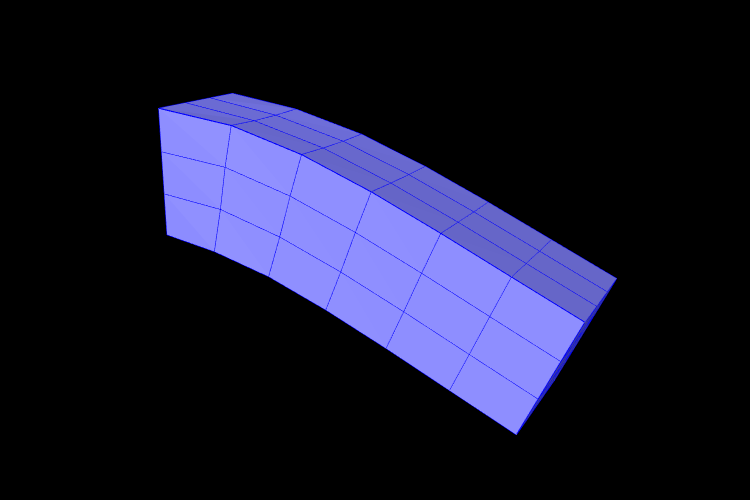
\includegraphics[width=\imglength]{images/FemBeam}
	\caption{FemBeam model loaded into ArtiSynth.}
	\label{fig:fem:beam}
\end{figure}

A complete application model that implements a simple FEM beam is given below.
\lstset{numbers=left}
\lstinputlisting{../../src/artisynth/demos/tutorial/FemBeam.java}
\lstset{numbers=none}
This example can be found in {\tt artisynth.demos.tutorial.FemBeam}.  The 
{\tt build()} method first creates a {\tt MechModel} and {\tt FemModel3d}.
A FEM beam is created using a factory method on line 36.  This beam is
centered at the origin, so its length extends from {\tt-length/2} to 
{\tt length/2}.  The density, damping and material properties are then 
assigned.  

On lines 45--49, a fixed boundary condition is set to the left-hand side 
of the beam by setting the corresponding nodes to be non-dynamic.  Due to 
numerical precision, a small {\tt EPSILON} buffer is required to ensure 
all left-hand boundary nodes are identified (line 46).

Rendering properties are then assigned to the FEM model on line 52.  These 
will be discussed further in Section \ref{sec:fem:rendering}.

\subsection{FEM Geometry}
\label{sec:fem:geometry}

Associated with each FEM model is a list of geometry with the heading 
{\tt meshes}.  This geometry can be used for either display purposes, 
or for interactions such as collisions.  A geometry itself has no 
physical properties; its motion is entirely governed by the FEM model 
that contains it.  

All FEM geometries are of type \javaclass[artisynth.core.femmodels]{FemMesh}, 
which stores a reference to a mesh object (Section \ref{Meshes:sec}), as well
as attachment information that links vertices of the mesh to points within
the FEM.  

\subsubsection{Surface meshes}

By default, every {\tt FemModel3d} has an auto-generated geometry representing
the ``surface mesh''.  The surface mesh consists of all un-shared element faces
(i.e.~the faces of individual elements that are exposed to the world), and its
vertices correspond to the nodes that make up those faces.  As the FEM nodes
move, so do the mesh vertices due to the attachment framework.

The surface mesh can be obtained using one of the following functions in 
{\tt FemModel3d}:
\begin{lstlisting}[]
FemMesh getSurfaceFemMesh ();     // returns the FemMesh surface component
PolygonalMesh getSurfaceMesh ();  // returns the underlying polygonal surface mesh
\end{lstlisting}
The first returns the surface complete with attachment information.  The latter 
method directly returns the {\tt PolygonalMesh} that is controlled by the FEM.  

It is possible to manually set the surface mesh:
\begin{lstlisting}[]
setSurfaceMesh ( PolygonalMesh surface );  // manually set surface mesh
\end{lstlisting}
However, doing so is normally not necessary.  It is always possible to add
additional mesh geometries to a finite element model, and the visibility
settings can be changed so that the default surface mesh is not rendered.  

\subsubsection{Embedding geometry within an FEM}

Any geometry of type \javaclass[maspack.geometry]{MeshBase} can be added to
a {\tt FemModel3d}.  To do so, first position the mesh so that its vertices 
are in the desired locations inside the FEM, then call one of the 
{\tt FemModel3d} methods:
\begin{lstlisting}[]
FemMesh addMesh ( MeshBase mesh );                // creates and returns FemMesh
FemMesh addMesh ( String name, MeshBase mesh );
\end{lstlisting}
The latter is a convenience routine that also gives the newly embedded
{\tt FemMesh} a name.

\subsubsection{Example: a beam with an embedded sphere}

\begin{figure}[ht]
	\centering
	\setlengthLaTeXML{\imglength}{0.8\textwidth}{0.6\textwidth}
	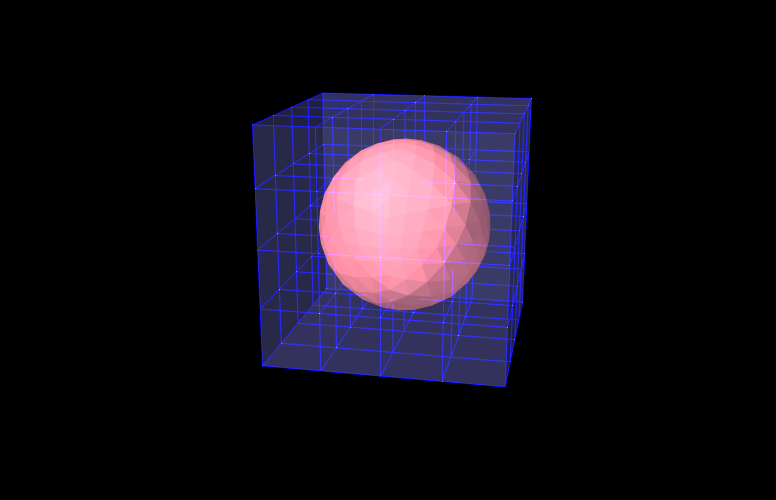
\includegraphics[width=\imglength]{images/FemEmbeddedSphere}
	\caption{FemEmbeddedSphere model loaded into ArtiSynth.}
	\label{fig:fem:embedded}
\end{figure}

A complete model demonstrating embedding a mesh is given below.
\lstset{numbers=left}
\lstinputlisting{../../src/artisynth/demos/tutorial/FemEmbeddedSphere.java}
\lstset{numbers=none}
This example can be found in {\tt artisynth.demos.tutorial.FemEmbeddedSphere}.
The model is very similar to {\tt FemBeam}.  A {\tt MechModel} and 
{\tt FemModel3d} are created and added.  At line 41, a {\tt PolygonalMesh}
of a sphere is created using a factory method.  The sphere is already
centered inside the beam, so it does not need to be repositioned.  At Line
42, the sphere is embedded inside model {\tt fem}, creating a {\tt FemMesh}
with the name ``sphere''.  The full model is shown in Figure 
\ref{fig:fem:embedded}.

\subsection{Node attachments}
\label{sec:fem:nodeattachments}

To couple FEM models to other dynamic components, an ``attachment'' mechanism 
is used.  Since \javaclass[artisynth.core.femmodels]{FemNode3d} 
is a subclass of \javaclass[artisynth.core.femmodels]{Particle}, the 
same attachment framework described in Section \ref{Attachments:sec} is 
available. FEM nodes can easily be connected to other dynamic objects, 
including other particles, nodes, and locations within elements.

\subsubsection{General principles}

To attach two components, a constraint system is established between their
velocities.  In general, this takes the form: 
%
\begin{equation}
\u_j = -\G_{j\alpha} \u_\alpha, \label{eqn:fem:attachment}
\end{equation}
%
where $\u_j$ and $\u_\alpha$ denote the velocities of the attached and
non-attached components.  The constraint matrix $G_{j\alpha}$ depends on
the types of components to be attached.  If attaching two points together, 
then $G_{j\alpha} = -I$.  For a point to a rigid body, $G_{j\alpha}$ will
depend on the current body location.  

An attachment is created in ArtiSynth by adding an object of type 
\javaclass[artisynth.core.mechmodels]{DynamicAttachment}.
Attachments involving a point (e.g.~{\tt FemNode3d}) extend the class 
\javaclass[artisynth.core.mechmodels]{PointAttachment}.  Common point-based
attachment classes are listed in Table \ref{tbl:fem:pointattachments}.
To add such an attachment constraint, create an object of the appropriate
type, and then add the attachment to the {\tt MechModel} using
\begin{lstlisting}[]
  addAttachment( DynamicAttachment attach ); // adds an attachment constraint
\end{lstlisting}
There are also convenience routines inside {\tt MechModel} that will create
the appropriate attachments automatically (see Section 
\ref{sec:mech:pointattachments}).

\begin{table}
	\centering
	\caption{Point-based attachments \label{tbl:fem:pointattachments}}

	\begin{tabular}{ll}
		\hline
		\hline
		Attachment & Description \\
		\hline
		\javaclass[artisynth.core.mechmodels]{PointParticleAttachment} & Attaches one ``point'' to one ``particle''\\
		\javaclass[artisynth.core.mechmodels]{PointFrameAttachment} & Attaches one ``point'' to one ``frame''\\
		\javaclass[artisynth.core.femmodels]{PointFem3dAttachment} &  Attaches one ``point'' to a linear combination of FEM nodes\\
		\hline
	\end{tabular}
\end{table}

\subsubsection{Example: connecting a beam to a block}

\begin{figure}[ht]
	\centering
	\setlengthLaTeXML{\imglength}{0.8\textwidth}{0.6\textwidth}
	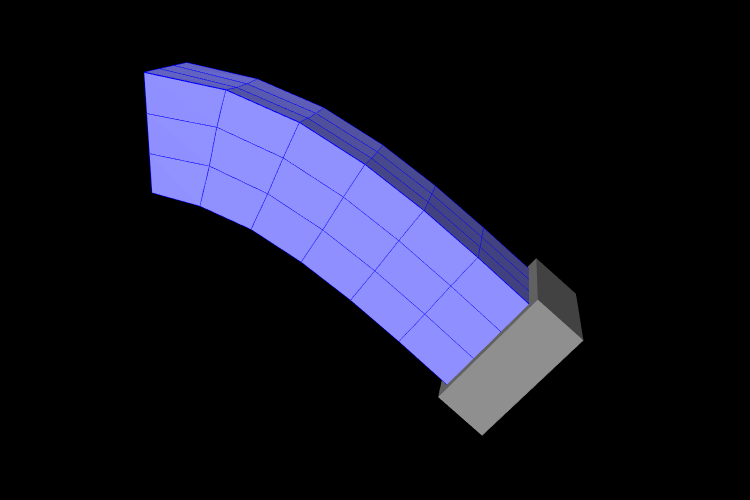
\includegraphics[width=\imglength]{images/FemBeamWithBlock}
	\caption{FemBeamWithBlock model loaded into ArtiSynth.}
	\label{fig:fem:beamwithblock}
\end{figure}

The following model demonstrates attaching a FEM beam to a rigid block.
\lstset{numbers=left}
\lstinputlisting{../../src/artisynth/demos/tutorial/FemBeamWithBlock.java}
\lstset{numbers=none}
This model extends the {\tt FemBeam} example of Section 
\ref{sec:fem:example:fembeam}.  The {\tt build()} method then creates 
and adds a {\tt RigidBody} block (lines 18--20).  One line 21, the block
is repositioned to the side of the beam to prepare for the attachment.
On lines 24--28, all right-most nodes of the beam are then set to be attached
to the block using a {\tt PointFrameAttachment}.  In this case, , the 
attachments are explicitly created.  They could also have been attached using
\begin{lstlisting}[]
   mech.attachPoint(node, block);  // attach node to rigid block
\end{lstlisting}



% FemBeamWithBlock

\subsubsection{Example: connecting two FEMs together}

% FemBeamWithFemSphere
\begin{figure}[ht]
	\centering
	\setlengthLaTeXML{\imglength}{0.8\textwidth}{0.6\textwidth}
	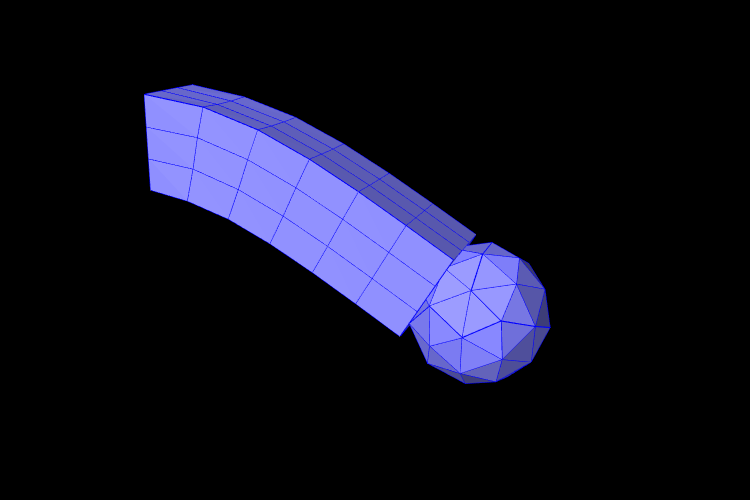
\includegraphics[width=\imglength]{images/FemBeamWithFemSphere}
	\caption{FemBeamWithFemSphere model loaded into ArtiSynth.}
	\label{fig:fem:beamwithfemsphere}
\end{figure}

The following model demonstrates how to attach two FEM models together:
\lstset{numbers=left}
\lstinputlisting{../../src/artisynth/demos/tutorial/FemBeamWithFemSphere.java}
\lstset{numbers=none}
This example can be found in 
{\tt artisynth.demos.tutorial.FemBeamWithFemSphere}.  The model extends 
{\tt FemBeam}, adding a finite element sphere and coupling them together.
The sphere is created and added on lines 18--28.  It is read from
TetGen-generated files using the 
\javaclass[artisynth.core.femmodels]{TetGenReader} class.  The model is then
scaled to match the dimensions of the current model, and transformed to the
right side of the beam.  To create attachments, the code first checks for 
any nodes that belong to the sphere that fall inside the beam using the
\javamethod[artisynth.core.femmodels]{FemModel3d.findContainingElement(Point3d)}
method (line 36), which returns the containing element if the point is inside
the model, or {\tt null} if the point is outside.  Internally, this spatial 
search uses a bounding volume hierarchy for efficiency (see 
\javaclass[maspack.geometry]{BVTree} and 
\javaclass[maspack.geometry]{BVFeatureQuery}).  If the point is contained
within the beam, then a {\tt PointFem3dAttachment} is implicitly added 
(line 39).

\subsection{FEM markers}

Just as there are {\tt FrameMarker}s to act as anchor points on a frame or
rigid body (Section \ref{FrameMarkers:sec}), there are also {\tt FemMarker}s 
that can mark a point inside a finite element.  They are frequently used to 
provide anchor points for attaching springs and forces to a point inside 
an element, but can also be used for graphical purposes.

FEM markers are implemented by the class
\javaclass[artisynth.core.femmodels]{FemMarker}, which
is a subclass of
\javaclass[artisynth.core.mechmodels]{Point}.
The following methods control the position and the element marked:
%
\begin{lstlisting}[]
  Point3d getPosition ();            // returns the current marker position
  void setPosition ( Point3d p );    // sets the current marker position

  FemElement3d getElement ();             // gets the current attached element
  void setElement ( FemElement3d elem )   // sets the current attached element
\end{lstlisting}
%
The positions are expressed in ``world coordinates''.  When a new position is
set, the marker automatically determines the ``natural coordinates'' coordinates
of the point within the its attached element.  Usually, the point falls inside
the element, however it is possible to add a marker outside the given element as
long as the shape functions are well-defined.  

Once a marker is created, it is added to the FEM model with the method
\begin{lstlisting}[]
  addMarker ( FemMarker marker );  // adds marker to this FemModel3d
\end{lstlisting}
A convenience method is also created that will automatically find the 
containing method:
\begin{lstlisting}[]
  FemMarker addMarker ( Point3d pos );  // creates and adds a FemMarker at pos
\end{lstlisting}
If the location is outside the model, it will be project to the nearest point
on the surface.  When a 3D force $\f$ is applied to the marker, 
it is distributed to the attached nodes according to the point's
natural coordinates within the element.  This guarantees conservation 
of power.

\subsubsection{Example: attaching a FEM beam to a muscle}

\begin{figure}[ht]
	\centering
	\setlengthLaTeXML{\imglength}{0.8\textwidth}{0.6\textwidth}
	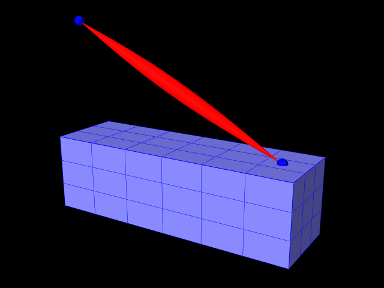
\includegraphics[width=\imglength]{images/FemBeamWithMuscle}
	\caption{FemBeamWithMuscle model loaded into ArtiSynth.}
	\label{fig:fem:beamwithmuscle}
\end{figure}

A complete application model that employs a fem marker as an anchor for a spring
is given below.
\lstset{numbers=left}
\lstinputlisting{../../src/artisynth/demos/tutorial/FemBeamWithMuscle.java}
\lstset{numbers=none}
This example can be found in {\tt artisynth.demos.tutorial.FemBeamWithMuscle}.
This model extends the {\tt FemBeam} example, adding a {\tt FemMarker} for the
spring to attach to.  The method {\tt createMarker(...)} on lines 28--34
is used to create and add a marker to the FEM.  Since the element is initially
set to {\tt null}, when it is added to the FEM, the model searches for the
containing or nearest element.  The loaded model is shown in Figure 
\ref{fig:fem:beamwithmuscle}.

% FemBeamWithMuscle

\subsection{Muscle activated FEM models}
\label{sec:fem:muscle}

Finite element muscle models are an extension to regular FEM models.  As such,
everything previously discussed for regular FEM models also applies to FEM
muscles.  Muscles have additional properties that allow them to contract when 
activated.  There are two types of muscles supported:
\begin{description}
\item[Fibre-based:] Point-to-point muscle fibres embedded in the model.
\item[Material-based:] An auxiliary material is added to the constitutive law
    to embed muscle properties. 
\end{description}
In this section, both types will be described.

\subsubsection{FemMuscleModel}

The class for FEM-based muscles is 
\javaclass[artisynth.core.femmodels]{FemMuscleModel}, a subclass 
of \javaclass[artisynth.core.femmodels]{FemModel3d}.  It differs from a basic
FEM model in that it has the new property
\begin{center}
	\begin{tabular}{|ll|}
		\hline
		Property & Description\\
		\hline
		{\tt muscleMaterial} & An object that adds an activation-dependent
		                       `muscle' term to the \emph{constitutive law}.\\
		\hline
	\end{tabular}
\end{center}
This is a delegate object of type 
\javaclass[artisynth.core.materials]{MuscleMaterial} that computes activation-%
dependent stress and stiffness in the muscle.  This property only applies to 
material-based muscles.  In addition, {\tt FemMuscleModel} has two more
lists of subcomponents:
\begin{description}
   \item[{\tt bundles}]\mbox{}\\
   Groupings of muscle sub-units (fibres or elements) that can be activated.

   \item[{\tt exciters}]\mbox{}\\
   Components that control the activation of a set of bundles or other exciters.
\end{description}

\paragraph{Bundles}
\ifLaTeXML{\newline}

Muscle bundles allow for a muscle to be partitioned into separate groupings
of fibres/elements, where each bundle can be activated independently.  They 
are implemented in the class \javaclass[artisynth.core.femmodels]{MuscleBundle}.
Bundles have three key properties:
\begin{center}
	\begin{tabular}{|ll|}
		\hline
		Property & Description\\
		\hline
		{\tt excitation} & Activation level of the muscle,  $a\in[0, 1]$.\\
		{\tt fibresActive} & Enable/disable ``fibre-based'' muscle components.\\
		{\tt muscleMaterial} & An object that adds an activation-dependent
		                       `muscle' term to the \emph{constitutive law}.\\
		\hline
	\end{tabular}
\end{center}
The {\tt excitation} property controls the level of muscle activation, with zero 
being no muscle action, and one being fully activated.  The {\tt fibresActive} 
property is a boolean variable that controls whether or not to treat any 
contained fibres as point-to-point-like muscles (``fibre-based'').  If false, 
the fibres are ignored.  The third property, {\tt muscleMaterial}, allows for a 
{\tt MuscleMaterial} to be specified per bundle.  By default, its value is 
inherited from {\tt FemMuscleModel}.

Once a muscle bundle is created, muscle sub-units must be assigned to it.  These
are either point-to-point fibres, or material-based muscle element descriptors.
The two types will be covered in Sections \ref{sec:fem:fibremuscle} and
\ref{sec:fem:materialmuscle}, respectively.

\paragraph{Exciters}
\ifLaTeXML{\newline}

Muscle exciters enable you to simultaneously activate a group of ``excitation 
components''.  This includes: point-to-point muscles, muscle bundles, muscle
fibre, material-based muscle elements, and other muscle exciters.  Components 
that can be excited all implement the 
\javaclass[artisynth.core.mechmodels]{ExcitationComponent}
interface.  To add or remove an component to the exciter, use
\begin{lstlisting}[]
  addTarget (ExcitationComponent ex);    // adds a component to the exciter
  addTarget (ExcitationComponent ex,     // adds a component with a gain factor
  	   double gain);   
  removeTarget (ExcitationComponent ex); // removes a component
\end{lstlisting}
If a gain factor is specified, the activation is scaled by the gain for that
component.

\subsubsection{Fibre-based muscles}
\label{sec:fem:fibremuscle}

In fibre-based muscles, a set of point-to-point muscle fibres are added between
FEM nodes or markers.  Each fibre is assigned an 
\javaclass[artisynth.core.materials]{AxialMuscleMaterial}, just like for 
regular point-to-point muscles (Section \ref{sec:mechii:musclematerials}).  Note
that these muscle materials typically have a ``rest length'' property, that will
likely need to be adjusted for each fibre.  Once the set of fibres are added
to a {\tt MuscleBundle}, they need to be enabled.  This is done by setting
the {\tt fibresActive} property of the bundle to {\tt true}.

Fibres are added to a {\tt MuscleBundle} using one of the functions:
\begin{lstlisting}[]
addFibre( Muscle muscle );              // adds a point-to-point fibre
Muscle addFibre( Point p0, Point p1,    // creates and adds a fibre
	 AxialMuscleMaterial mat);
\end{lstlisting}
The latter returns the newly created {\tt Muscle} fibre.

The following code snippet demonstrates how to create a fibre-based {\tt MuscleBundle}
and add it to a FEM muscle.
\lstset{numbers=left}
\begin{lstlisting}[]
// Create a muscle bundle
MuscleBundle bundle = new MuscleBundle("fibres");
Point3d[] fibrePoints = ...   //create a sequential list of points

// Add fibres
Point pPrev = fem.addMarker(fibrePoints[0]);    // create a FEM marker
for (int i=1; i<=fibrePoints.length; i++) {
   Point pNext = fem.addMarker(fibrePoint[i]);

   // Create fibre material
   double l0 = pNext.distance(pPrev);           // rest length
   AxialMuscleMaterial fibreMat = 
         new BlemkerAxialMuscle(
               1.4*l0, l0, 3000, 0, 0);

   // Add a fibre between pPrev and pNext
   bundle.addFibre(pPrev, pNext, fibreMat);     // add fibre to bundle
   pPrev = pNext;
}

// Enable use of fibres (default is disabled)
bundle.setFibresActive(true);
fem.addMuscleBundle(bundle);                    // add the bundle to fem
\end{lstlisting}
\lstset{numbers=none}

In these fibre-based muscles, force is only exerted between the anchor
points of the fibres; it is a discrete approximation.  These models
are typically more stable than material-based ones.

\subsubsection{Material-based muscles}
\label{sec:fem:materialmuscle}

In material-based muscles, the constitutive law is augmented with additional
terms to account for muscle-specific properties.  This is a continuous 
representation within the model.  

The basic building block for a material-based muscle bundle is a 
\javaclass[artisynth.core.femmodels]{MuscleElemDesc}.  This object contains
a reference to a {\tt FemElement3d}, a {\tt MuscleMaterial}, and either a
single direction or set of directions that specify the direction of 
contraction.  If a single direction is specified, then it is assumed the
entire element contracts in the same direction.  Otherwise, a direction
can be specified for each \emph{integration point} within the element.  A
{\tt null} direction signals that there is no muscle at the corresponding
point.  This allows for a sub-element resolution for muscle definitions. The 
positions of integration points for a given element can be obtained with:
\begin{lstlisting}[]
// loop through all integration points for a given element
for ( IntegrationPoint3d ipnt : elem.getIntegrationPoints() ) {
	Point3d curPos = new Point3d();
	Point3d restPos = new Point3d();
	ipnt.computePosition (curPos, elem);          // computes current position
	ipnt.computeRestPosition (restPos, elem);     // computes rest position
}
\end{lstlisting} 
By default, the {\tt MuscleMaterial} is inherited from the bundle's 
{\tt material} property.  Supported muscle materials include:
\javaclass[artisynth.core.materials]{GenericMuscle}, 
\javaclass[artisynth.core.materials]{BlemkerMuscle}, and 
\javaclass[artisynth.core.materials]{FullBlemkerMuscle}.  The Blemker-type
materials are based on \cite{blemker:2005:muscle}.  {\tt BlemkerMuscle} only
uses the muscle-specific terms (since a base material is provided the 
underlying FEM model).  {\tt FullBlemkerMuscle} adds all terms described in 
the paper.

Elements can be added to a muscle bundle using one of the methods:
\begin{lstlisting}[]
// Adds a muscle element
addElement (MuscleElementDesc elem);          
// Creates and adds a muscle element
MuscleElemDesc addElement (FemElement3d elem, Vector3d dir);     
// Sets a direction per integration point
MuscleElemDesc addElement (FemElement3d elem, Vector3d[] dirs);  
\end{lstlisting}

The following snippet demonstrates how to create and add a material-based
muscle bundle:
\lstset{numbers=left}
\begin{lstlisting}[]
// Create muscle bundle
MuscleBundle bundle = new MuscleBundle("embedded");

// Muscle material
MuscleMaterial muscleMat = new BlemkerMuscle(
      1.4, 1.0, 3000, 0, 0);
bundle.setMuscleMaterial(muscleMat); 

// Muscle direction
Vector3d dir = Vector3d.X_UNIT;

// Add elements to bundle
for (FemElement3d elem : beam.getElements()) {
   bundle.addElement(elem, dir);
}

// Add bundle to model      
beam.addMuscleBundle(bundle);
\end{lstlisting}
\lstset{numbers=none}

\subsubsection{Example: comparison with two beam examples}

\begin{figure}[ht]
	\centering
	\setlengthLaTeXML{\imglength}{0.8\textwidth}{0.6\textwidth}
	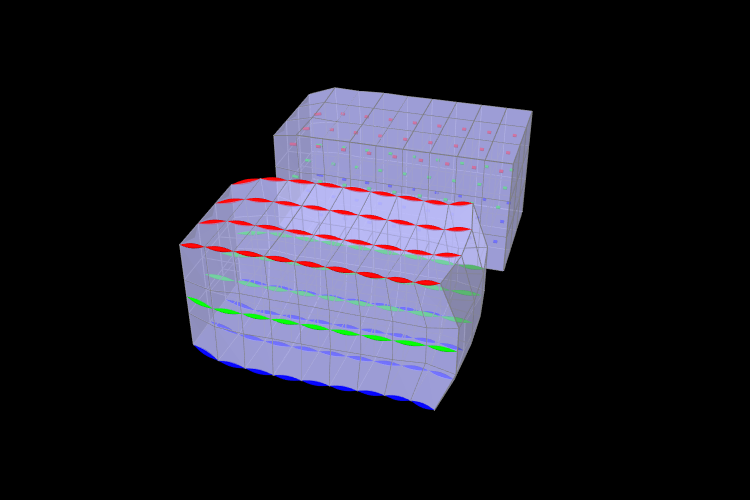
\includegraphics[width=\imglength]{images/FemMuscleBeamsContracted}
	\caption{FemMuscleBeams model loaded into ArtiSynth.}
	\label{fig:fem:musclebeams}
\end{figure}

% FemMuscleBeams
An example comparing a fibre-based and a material-based muscle is shown 
in Figure \ref{fig:fem:musclebeams}.  The code can be found in 
{\tt artisynth.demos.tutorial.FemMuscleBeam}.  There are two 
{\tt FemMuscleModel} beams in the model: one fibre-based, and one 
material-based.  Each has three muscle bundles: one at the top (red),
one in the middle (green), and one at the bottom (blue).  In the figure,
both muscles are fully activated.  Note the deformed shape of the beams.
In the fibre-based one, since forces only act between point on the fibres,
the muscle seems to bulge.  In the material-based muscle, the entire
continuous volume contracts, leading to a uniform deformation.  

Material-based muscles are more realistic.  However, it comes at the cost
of stability.  The added terms to the constitutive law are highly non-linear,
which may cause numerical issues as elements become highly contracted or
highly deformed.  Fibre-based muscles are, in general, more stable.  However,
they can lead to bulging and other deformation artifacts due to their discrete
nature.

\subsection{Collisions}
\label{sec:fem:collision}

As described in Section \ref{sec:mechii:collisions}, collisions can be enabled 
for any class that implements the 
\javaclass[artisynth.core.mechmodels]{Collidable} interface.  Both 
\javaclass[artisynth.core.femmodels]{FemModel3d} and 
\javaclass[artisynth.core.femmodels]{FemMesh} implement 
\javaclass[artisynth.core.mechmodels]{Collidable}.  {\tt FemModel3d}
will use its surface mesh as the collision surface.  A {\tt FemMesh} will use
its underlying mesh structure.  At present, only meshes of type 
\javaclass[maspack.geometry]{PolygonalMesh} are supported.

Since {\tt FemMesh} is also a {\tt Collidable}, this means we can enable 
collisions with any embedded mesh inside a FEM.  Any forces resulting from
the collision are then transfered back to the underlying nodes of the model.

\subsubsection{Example: FEM collisions}

\begin{figure}[ht]
	\centering
	\setlengthLaTeXML{\imglength}{0.8\textwidth}{0.6\textwidth}
	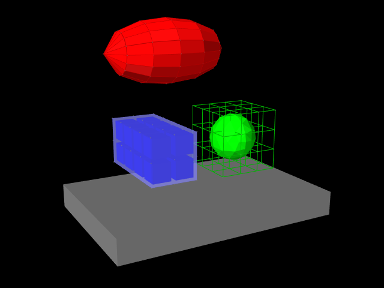
\includegraphics[width=\imglength]{images/FemCollisions}
	\caption{FemCollisions model loaded into ArtiSynth.}
	\label{fig:fem:collisions}
\end{figure}

An example of FEM collisions is shown in Figure \ref{fig:fem:collisions}.
The full source code can be found in the ArtiSynth repository under
{\tt artisynth.demos.tutorial.FemCollisions}.  The collision-enabling
code is as follows:
\begin{lstlisting}[]
// Set up collisions
mech.setCollisionBehavior(ellipsoid, beam, true);   // beam-ellipsoid
mech.setCollisionBehavior(ellipsoid, table, true);  // ellipsoid-table
mech.setCollisionBehavior(table, beam, true);       // beam-table

FemMesh embeddedSphere = block.getMesh("embedded");      // get embedded FemMesh
mech.setCollisionBehavior(embeddedSphere, table, true);      // sphere-table
mech.setCollisionBehavior(ellipsoid, embeddedSphere, true);  // sphere-ellipsoid   
\end{lstlisting}
Notice in the figure that the surface of the green block passes through
the table and ellipsoid; only the embedded sphere has collisions enabled.

\subsection{Rendering and Visualizations}
\label{sec:fem:rendering}

In addition to the standard {\tt RenderProps} that control how the
nodes and surfaces appear, finite element models and their sub-components
have a few additional properties that affect rendering.  Some of these
are listed in Table \ref{tbl:fem:rendering}.

\begin{table}[ht]
	\centering
	\caption{FEM-specific rendering properties} \label{tbl:fem:rendering}
	\begin{tabular}{lp{0.5\textwidth}}
		\hline\hline
		Property & Description\\
		\hline
	   {\tt elementWidgetSize} & size of element to render $\in [0,1]$\\
	   {\tt directionRenderLen} & relative length to draw fibre direction indicator $\in [0, 1]$\\
	   {\tt directionRenderType} & where to draw directions: {\tt ELEMENT}, {\tt INTEGRATION\_POINT}\\
	   {\tt surfaceRendering} & how to render surface: {\tt None}, {\tt Shaded}, {\tt Stress}, {\tt Strain}\\
	   {\tt stressPlotRange} & range of values for stress/strain plot\\
	   {\tt stressPlotRanging} & how to determine stress/strain plot range: {\tt Auto}, {\tt Fixed}\\
	   {\tt colorMap} & delegate object controlling the map of stress/strain values to color\\
	   \hline
	\end{tabular}
\end{table}

The property {\tt elementWidgetSize} applies only to 
\javaclass[artisynth.core.femmodels]{FemModel3d} and
\javaclass[artisynth.core.femmodels]{FemElement3d}.  It specifies the scale to
draw each element volume.  For instance, the blue beam in Figure \ref{fig:fem:collisions}
uses a widget size of 0.8, resulting in a mosaic-like pattern.

The next two properties in Table \ref{tbl:fem:rendering} apply to the muscle classes 
\javaclass[artisynth.core.femmodels]{FemMuscleModel}, 
\javaclass[artisynth.core.femmodels]{MuscleBundle}, and
\javaclass[artisynth.core.femmodels]{MuscleElemDesc}.
When {\tt directionRenderLen > 0}, lines are drawn inside elements to indicate fibre
directions.  If {\tt directionRenderType = ELEMENT}, then one line is drawn per
element indicating the average contraction direction.  If 
{\tt directionRenderType = INTEGRATION\_POINT}, a separate line is drawn per point.

The last four properties apply to 
\javaclass[artisynth.core.femmodels]{FemModel3d} and 
\javaclass[artisynth.core.femmodels]{FemMesh}.
They control how the surface is colored.  This can be used to enable stress/strain
visualizations.  The property {\tt surfaceRendering} sets what to draw:\\
\begin{tabular}{lll}
& {\tt None} & no surface\\
& {\tt Shaded} & the face color specified by the mesh's {\tt RenderProps}\\
& {\tt Stress} & the von Mises stress\\
& {\tt Strain} & the von Mises strain
\end{tabular}
The {\tt stressPlotRange} controls the range of values to use when plotting 
stress/strain.  Values outside this range are truncated.  The {\tt colorMap}
is a delegate object that converts those stress and strain values to colors.
Various types of maps exist, including 
\javaclass[maspack.render.color]{GreyscaleColorMap},
\javaclass[maspack.render.color]{HueColorMap},
\javaclass[maspack.render.color]{RainbowColorMap}, and
\javaclass[maspack.render.color]{JetColorMap}.  These all implement the
\javaclass[maspack.render.color]{ColorMap} interface.

To display values corresponding to colors, a 
\javaclass[artisynth.core.renderables]{ColorBar} needs to be added to the 
{\tt RootModel}.  Color bars are general {\tt Renderable} objects that are
only used for visualizations.  They are added to the display using the
\begin{lstlisting}[]
addRenderable (Renderable r);
\end{lstlisting}
method in {\tt RootModel}.  Color bars also have a {\tt ColorMap} associated
with it.  The following functions are useful for controlling its visualization:
\begin{lstlisting}[]
setNumberFormat ( String fmtStr );    // C-like numeric format specification
populateLabels ( double min, double max, int tick );     // initialize labels
updateLabels ( double min, double max );                 // update existing labels

setColorMap ( ColorMap map );                            // set color map

// Control position/size of the bar
setNormalizedLocation (double x, double y, double width, double height);
setLocationOverride (double x, double y, double width, double height)
\end{lstlisting}
The normalized location specifies sizes relative to the screen size 
(1 = screen width/height).  The location override, if values are non-zero,
will override the normalized location, specifying values in absolute pixels.
Negative values for position correspond to distances from the left/top.
For instance,
\begin{lstlisting}[]
setNormalizedLocation(0, 0.1, 0, 0.8);
setLocationOverride(-40, 0, 20, 0);
\end{lstlisting}
will create a bar that is 10\% up from the bottom of the screen, 40 pixels from
the right edge, with a height occupying 80\% of the screen, and width 20 pixels.

Note that the color bar is not associated with any mesh or finite element model.
Any synchronization of colors and labels must be done manually by the developer.
It is recommended to do this in the {\tt RootModel}'s {\tt prerender(...)} method,
so that colors are updated every time the model's rendering configuration changes.

\subsubsection{Example: stress and strain plotting}

\begin{figure}[ht]
	\centering
	\setlengthLaTeXML{\imglength}{0.8\textwidth}{0.6\textwidth}
	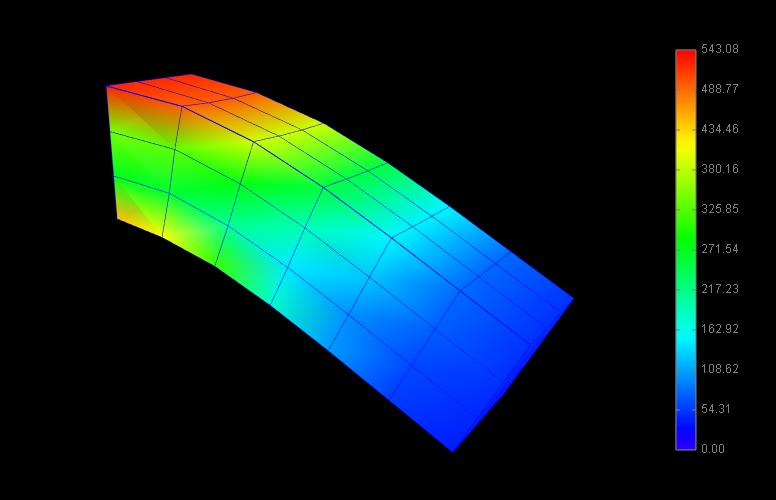
\includegraphics[width=\imglength]{images/FemBeamColored}
	\caption{FemBeamColored model loaded into ArtiSynth.}
	\label{fig:fem:beamcolored}
\end{figure}

The following model extends {\tt FemBeam} to render stress, with an added 
color bar.  The loaded model is shown in Figure \ref{fig:fem:beamcolored}.
\lstset{numbers=left}
\lstinputlisting{../../src/artisynth/demos/tutorial/FemBeamColored.java}
\lstset{numbers=none}
